\documentclass[10pt,a4paper]{article}
\usepackage[margin=2.1cm]{geometry}
\usepackage[T1]{fontenc}
\usepackage{lmodern}
\usepackage{microtype}
\usepackage{graphicx}
\usepackage{amsmath}
\usepackage{booktabs}
\usepackage{tabularx}
\usepackage{multirow}
\usepackage{float}
\usepackage{xcolor}
\usepackage{titlesec}
\usepackage{fancyhdr}
\usepackage[colorlinks=true,linkcolor=blue!50!black,urlcolor=blue!50!black,citecolor=blue!50!black]{hyperref}

\graphicspath{{figures/}}
\titleformat{\section}{\large\bfseries}{\thesection}{0.6em}{}
\titleformat{\subsection}{\normalsize\bfseries}{\thesubsection}{0.6em}{}
\setlength{\parskip}{0.35em}
\setlength{\parindent}{0pt}
\pagestyle{fancy}
\fancyhf{}
\lhead{\small Counting Challenge -- Om Rode}
\rhead{\small \thepage}
\renewcommand{\headrulewidth}{0.3pt}
\makeatletter\newcommand{\tabinput}[1]{\@@input #1 }\makeatother
\newcommand{\code}[1]{\texttt{\small #1}}

\title{\textbf{Counting Challenge}\\[0.3em]\large Object counting with instance masks: a classical (Non-AI) and a learned (AI) solution}
\author{Om Rode}
\date{November 2026}

\begin{document}
\maketitle
\thispagestyle{fancy}

\begin{abstract}
\noindent
The task is to count the screws, bolts, discs and nuts in 25 photographs and overlay one mask per object, with an accuracy above 95\,\%.
Two independent solutions were built.
The \textbf{Non-AI} solution uses classical OpenCV operations: illumination flattening, Otsu thresholding, round-hole detection for nuts, a disc model based on the distance transform, and area-based cluster counting with watershed splitting.
The \textbf{AI} solution is a YOLOv8s-seg instance-segmentation model, fine-tuned on labels generated automatically with SAM~2.1.
An automatic audit pointed a human only at suspicious spots; 16 objects in 8 images were corrected with one click each.
Count accuracy is $1-|\hat{n}-n|/n$ per image.
The Non-AI solution reaches \textbf{99.7\,\%} mean accuracy over all images (worst image 98.0\,\%).
The AI solution reaches \textbf{99.9\,\%} on the five held-out test images and 99.4\,\% over all images (worst image 95.2\,\%).
\end{abstract}

% ---------------------------------------------------------------------------
\section{Dataset and ground truth}

The dataset has 25 photographs of metal parts on a plain background, in two groups (Figure~\ref{fig:dataset}):
\begin{itemize}\setlength{\itemsep}{0pt}
  \item \code{Screws\_2024\_07\_15}: seven $1920\times1080$ shots of the same 43 screws. The file name \code{img1\_43\_nosy} gives the count.
  \item \code{ScrewAndBolt\_20240713}: eighteen $3000\times4000$ phone photos. They show a few screws (10 and 21), dense piles of countersunk screws (about 193), screws mixed with discs (about 98), and a pile of 354 hex nuts.
\end{itemize}

\begin{figure}[H]
  \centering
  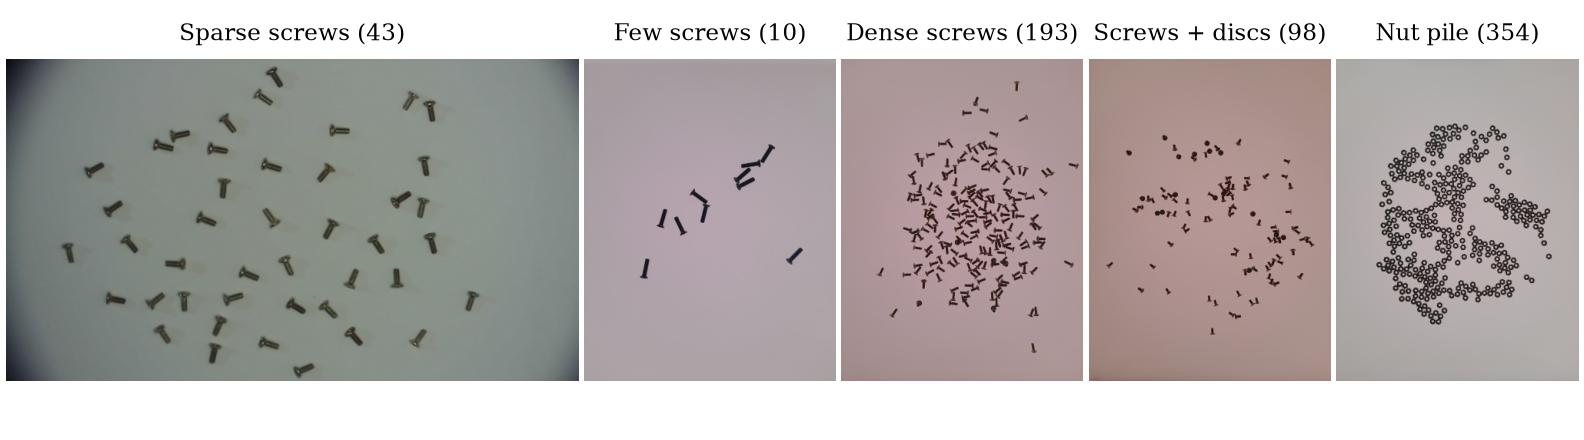
\includegraphics[width=\linewidth]{dataset.jpg}
  \caption{One image of each scene type. These five images form the held-out test split of the AI model.}
  \label{fig:dataset}
\end{figure}

\textbf{Ground truth.} The dataset has no labels, so the ground truth (\code{Om\_Rode/ground\_truth.csv}) was built from these sources, which agree with each other:
\begin{itemize}\setlength{\itemsep}{0pt}
  \item manual counts of the sparse images, and the ``43'' in the file name;
  \item the number of round nut holes, which is the same in all five nut photos (354);
  \item the SAM auto-labels, checked by the audit and corrected where needed (Section~\ref{sec:labels}), then approved on a review page.
\end{itemize}

% ---------------------------------------------------------------------------
\section{Non-AI solution (OpenCV)}

\code{Non\_AI/count\_objects.py} has no learned parameters. It processes one image in about 0.4\,s on a CPU.

\subsection{Foreground segmentation}
\begin{enumerate}\setlength{\itemsep}{0pt}
  \item The image is resized to a long side of 1600\,px, so that all kernel sizes are the same for every photo.
  \item \textbf{Illumination flattening.} The background is estimated with a grey-level closing ($41\times41$ ellipse), which removes the dark objects, followed by a large Gaussian blur. The image is divided by this estimate. This removes uneven lighting and lens vignetting (Figure~\ref{fig:nonai}b).
  \item \textbf{Otsu threshold} on the flattened image, a $3\times3$ opening and closing, and hole filling (Figure~\ref{fig:nonai}c).
  \item \textbf{Valid field of view.} Blobs that are more than 30\,\% inside the black vignette corners are removed.
\end{enumerate}

\begin{figure}[H]
  \centering
  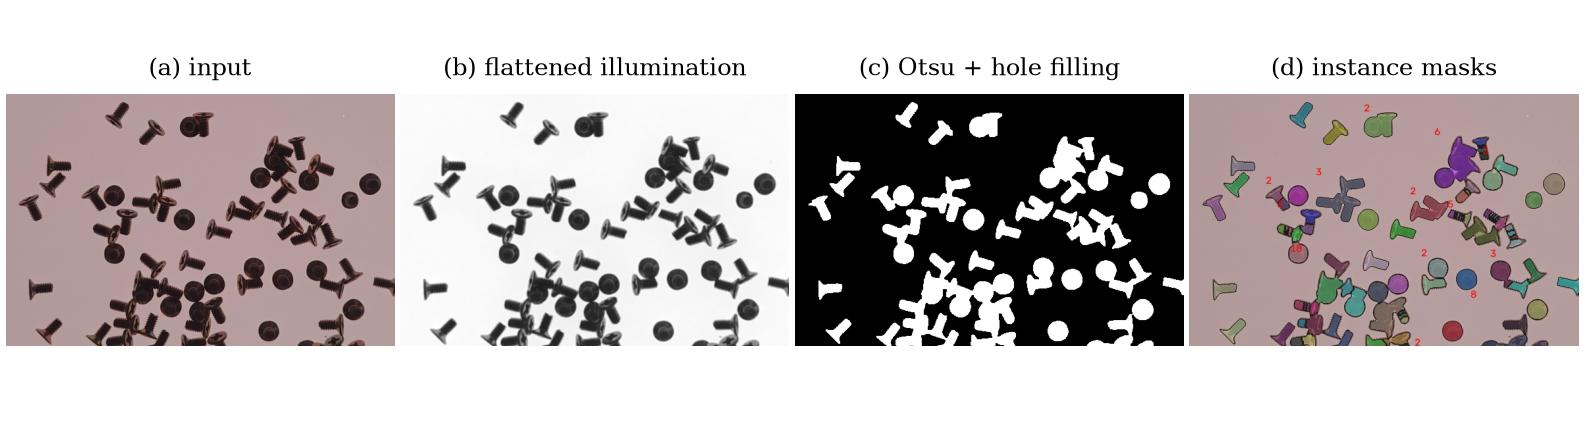
\includegraphics[width=\linewidth]{nonai_steps.jpg}
  \caption{Non-AI pipeline on a screws-and-discs image (crop). (d) shows one coloured mask per counted object; a red number is the count given to a cluster.}
  \label{fig:nonai}
\end{figure}

\subsection{Counting}

\textbf{Nuts: one round hole is one nut.}
The inner contours of the thresholded image are the holes. A hole counts if it is round (circularity $4\pi A/P^2 > 0.75$) and between 0.4 and 2 times the median hole area. Gaps that are enclosed between touching parts are irregular, so they fail the circularity test.
A blob with $k$ round holes contains $k$ nuts. Each pixel of the blob is assigned to its nearest hole centre, which splits the blob into $k$ masks (a Voronoi split, Figure~\ref{fig:nuts}).
On the five nut photos this gives 353--355 against a ground truth of 354.

\begin{figure}[H]
  \centering
  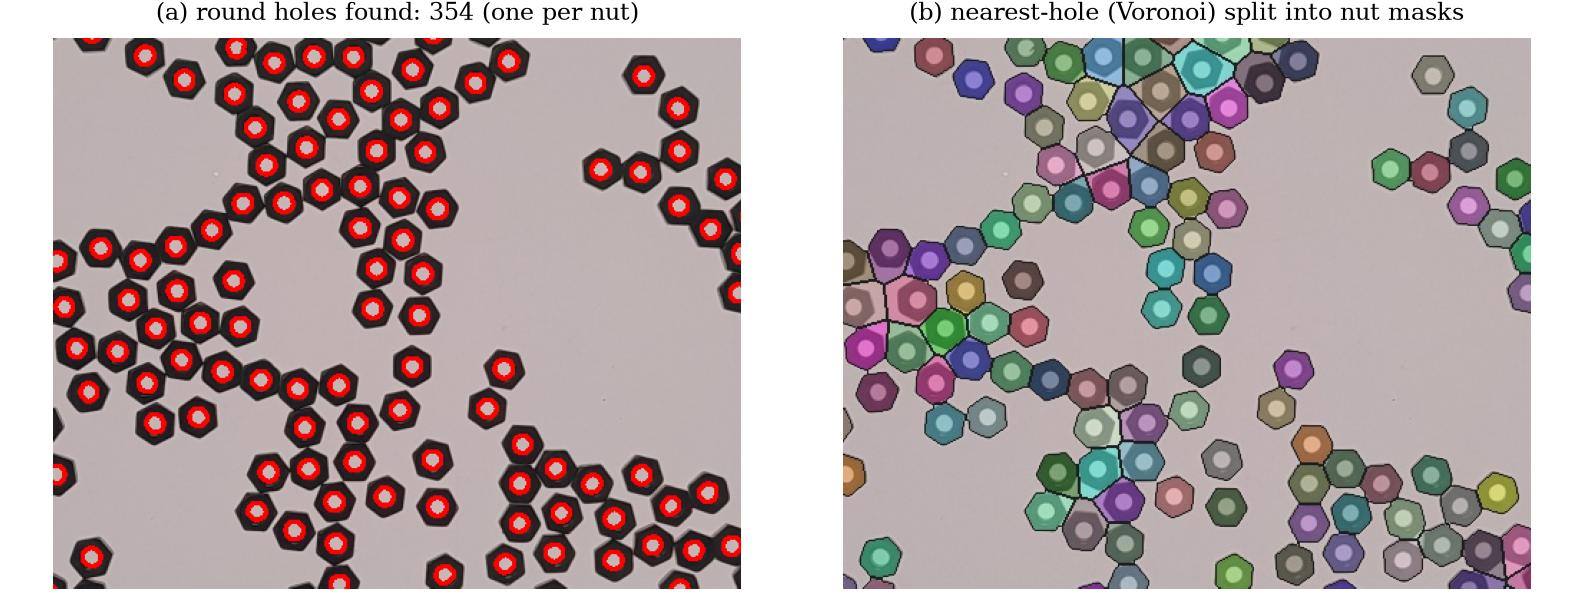
\includegraphics[width=\linewidth]{nonai_nuts.jpg}
  \caption{Nut pile (crop). (a) Detected round holes. (b) Nut masks after the nearest-hole split.}
  \label{fig:nuts}
\end{figure}

\textbf{Screws and discs.}
\begin{itemize}\setlength{\itemsep}{0pt}
  \item The \emph{single-object area} $a_1$ is the left-most strong mode of the log-area histogram of all blobs. The median does not work, because in sparse scenes most blobs are touching pairs.
  \item \emph{Discs} have about 1.3 times the area of a screw. Isolated round blobs (circularity $> 0.8$) give the disc area $a_d$ and radius $r$. Inside any blob, each region where the distance transform is at least $0.8\,r$ is one disc (Figure~\ref{fig:discs}). Screw heads and shanks are much thinner, so they do not produce such regions.
  \item The count of a blob is
  \[
    k = n_d + \mathrm{round}\!\left(\frac{A - n_d\,a_d}{a_1\cdot c}\right),
    \qquad c = \begin{cases}1.06 & \text{if the blob holds more than 2.5 objects}\\ 1 & \text{otherwise}\end{cases}
  \]
  where $A$ is the blob area and $n_d$ the number of discs. The crowding factor $c$ was measured: in clusters of three or more objects, the area per object is 1.05--1.07 times $a_1$, because shadows and blurred edges between touching objects add area.
  \item A cluster is split into $k$ masks with a distance-transform watershed.
\end{itemize}

\begin{figure}[H]
  \centering
  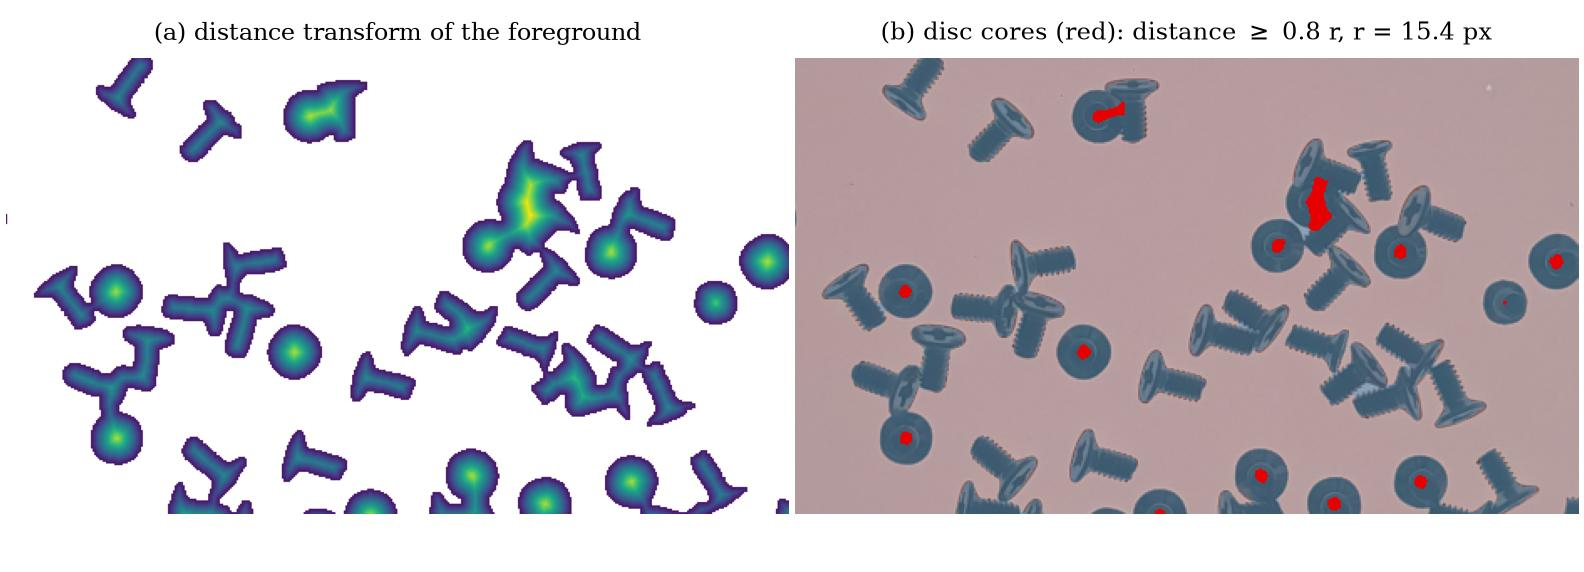
\includegraphics[width=\linewidth]{nonai_discs.jpg}
  \caption{Disc detection inside clusters. Only discs have a distance-transform core thicker than $0.8\,r$ (red). Two touching discs give one elongated core, which is counted as two.}
  \label{fig:discs}
\end{figure}

Before the disc model and the crowding factor were added, every disc was counted as about 1.3 objects. The screws-and-discs images then scored only 84--94\,\%. With both changes, the worst image is at 98\,\%.

% ---------------------------------------------------------------------------
\section{AI solution (YOLOv8s-seg trained on SAM~2.1 labels)}

\subsection{Automatic labelling with SAM 2.1}\label{sec:labels}

\code{AI/autolabel\_sam.py} produces instance labels without manual drawing:
\begin{enumerate}\setlength{\itemsep}{0pt}
  \item The image is resized to a long side of 2400\,px. SAM~2.1-base runs in ``segment everything'' mode on $1024\times1024$ tiles with stride 768. Masks that touch an interior tile edge are dropped, because the neighbouring tile sees those objects whole.
  \item \textbf{Clean-up:}
  \begin{itemize}\setlength{\itemsep}{0pt}
    \item duplicate masks are removed by IoU;
    \item a mask is kept only if it lies on the Non-AI foreground and inside the valid field of view;
    \item group masks and part masks are resolved;
    \item fragments smaller than $0.2\times$ the median object area are removed.
  \end{itemize}
  \item \textbf{Recovery of missed objects (up to 3 rounds).} Each uncovered thick dark region is prompted with a point. If that fails, it is prompted with a point and a box. If the region is still too large, it gets one prompt per distance-transform peak, with the other peaks as negative points.
  \item \textbf{Merging parts.} SAM often returns a pan-head screw as two masks (head and shank). Adjacent parts whose combined area is close to one object are merged.
\end{enumerate}
The labels are stored as YOLO polygons, as compressed masks for the audit, and as overlays (Figure~\ref{fig:samov}).

\begin{figure}[H]
  \centering
  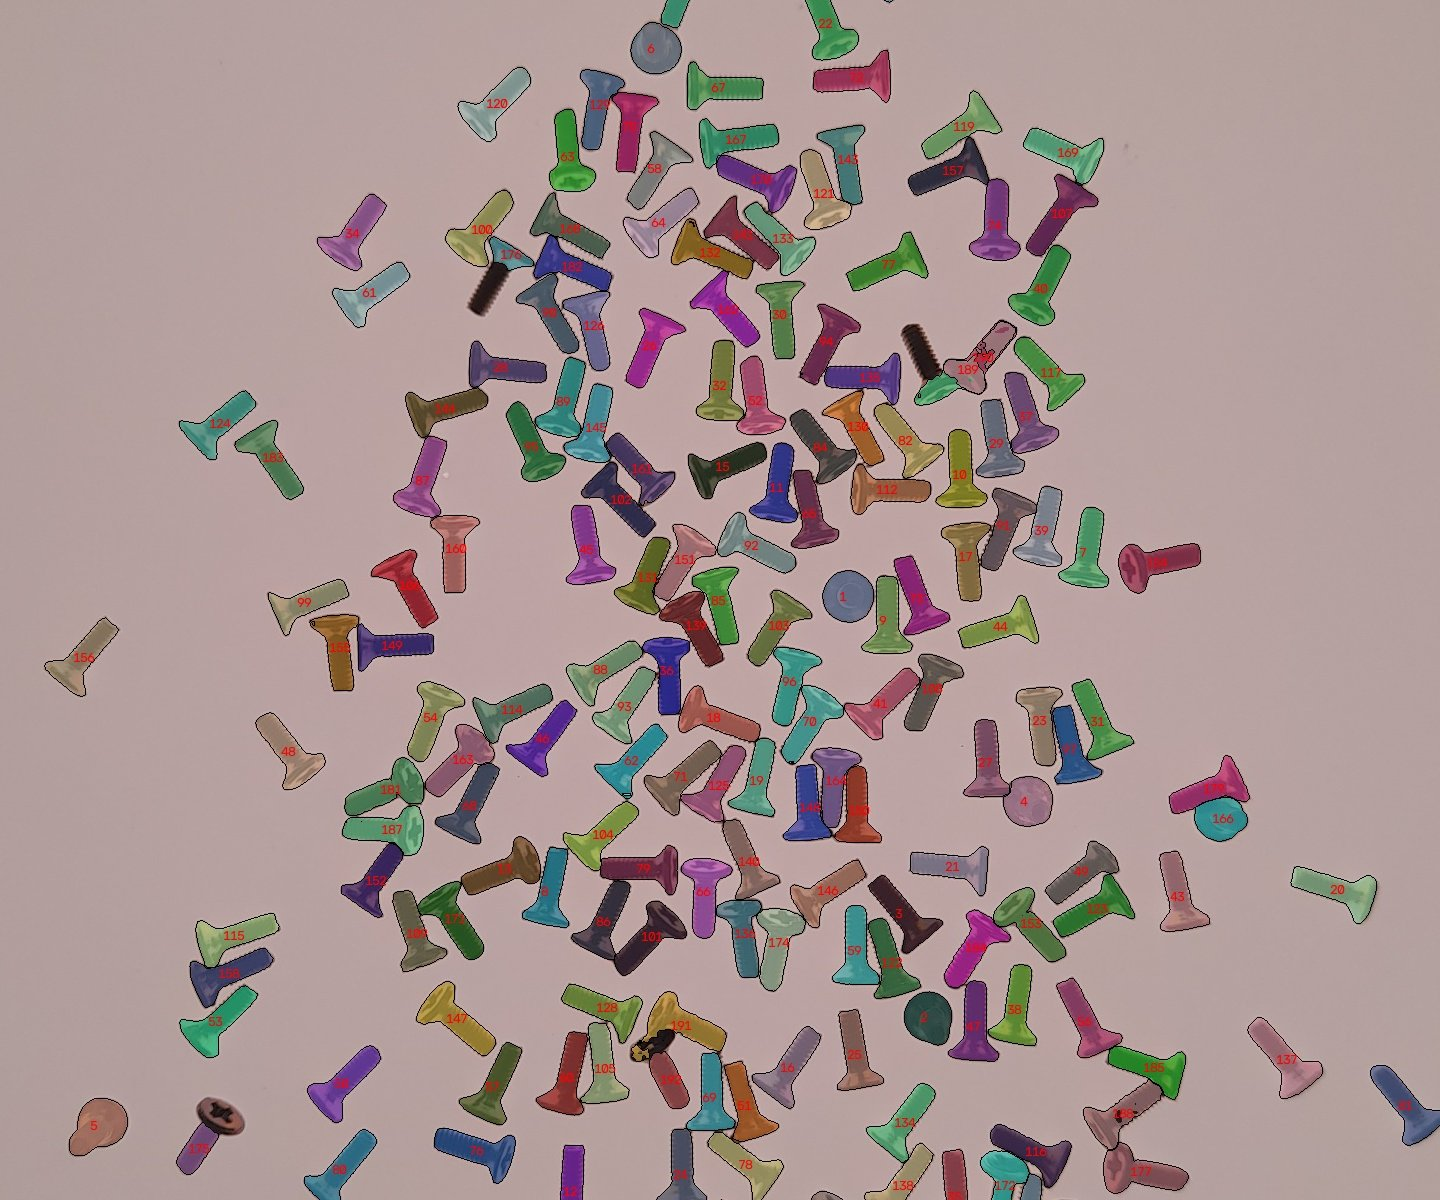
\includegraphics[width=0.62\linewidth]{sam_overlay.jpg}
  \caption{Final SAM labels for a dense screw image (crop). Each colour is one instance.}
  \label{fig:samov}
\end{figure}

\subsection{Audit and minimal human correction}

\code{AI/audit\_labels.py} compares the labels with independent classical signals and flags these cases:
\begin{itemize}\setlength{\itemsep}{0pt}
  \item \emph{possible miss}: a thick foreground blob with no mask;
  \item \emph{possible merge}: a mask larger than $1.6\times$ the median area;
  \item a mismatch with the number of nut holes or with the Non-AI count.
\end{itemize}
Only the flagged spots were reviewed. 16 of them were real errors: 12 merges and 4 misses. The others were harmless, for example a screw head masked without its shank, which does not change the count.
Each error was fixed with one click in \code{corrections.json}, applied by \code{apply\_corrections.py}:
\begin{itemize}\setlength{\itemsep}{0pt}
  \item \code{add}: a SAM point prompt at the click;
  \item \code{split}: one prompt per distance-transform peak of the merged mask, with the other peaks as negative points.
\end{itemize}
Table~\ref{tab:corr} lists the corrections and Figure~\ref{fig:corr} shows two of them.
17 of the 25 images needed no correction. Before correction, the SAM count was 0.9\,\% from the final count on average, over the 18 phone photos.

\begin{table}[H]
  \centering
  \small
  \caption{One-click label corrections. All other images were correct automatically.}
  \label{tab:corr}
  \begin{tabular}{llrrrr}
    \toprule
    Code & Image & Adds & Splits & SAM automatic & After review \\
    \midrule
    \tabinput{tables/corrections.tex}
    \midrule
    \multicolumn{2}{l}{Total (8 images)} & 4 & 12 & & \\
    \bottomrule
  \end{tabular}
\end{table}

\begin{figure}[H]
  \centering
  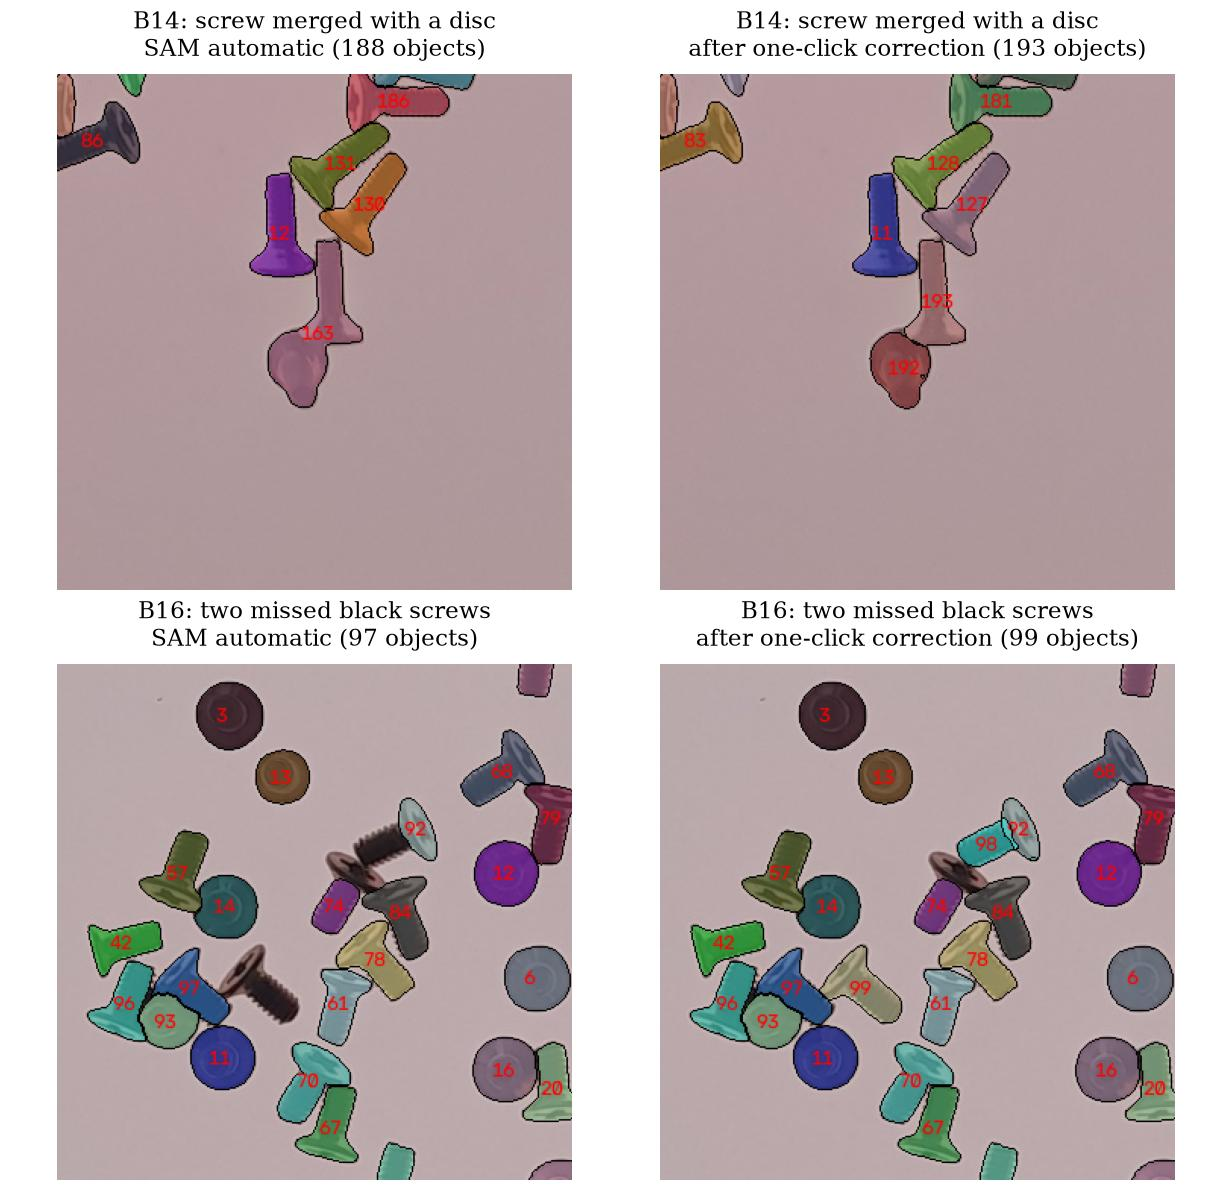
\includegraphics[width=0.78\linewidth]{sam_correction.jpg}
  \caption{Two corrections. Top: a screw merged with a disc is split with two prompts. Bottom: two black screws that SAM missed are added with one point each.}
  \label{fig:corr}
\end{figure}

\subsection{Dataset and training}

\textbf{Split by image}, so that no tiles of a test image are used in training:
\begin{itemize}\setlength{\itemsep}{0pt}
  \item test: one image per scene type (Figure~\ref{fig:dataset});
  \item validation: \code{img6} and \code{194206};
  \item train: the remaining 18 images.
\end{itemize}
The training images are cut into $1024\times1024$ tiles with stride 512, at the 2400\,px scale used for inference. This gives 182 tiles. An object cut by a tile border is kept if at least 40\,\% of it is visible.
Table~\ref{tab:train} lists the training settings and Figure~\ref{fig:train} the training curves.

\begin{table}[H]
  \centering
  \small
  \caption{Training configuration (\code{AI/train.py}).}
  \label{tab:train}
  \begin{tabularx}{0.9\linewidth}{lX}
    \toprule
    Model & YOLOv8s-seg, COCO-pretrained, 11.8\,M parameters, 1 class (\emph{object}) \\
    Input & $1024\times1024$ tiles, batch 1 \\
    Epochs & at most 120, early stopping with patience 40; stopped at epoch 86, best weights from epoch 46 \\
    Augmentation & rotation $\pm180^\circ$, horizontal and vertical flips, scale $\pm40\,\%$, translation 0.1, HSV jitter; mosaic off \\
    Other & \code{max\_det=1000}, \code{overlap\_mask=True}, seed 0 \\
    Hardware & NVIDIA RTX 3050 Laptop (6\,GB); 29\,min of training \\
    \bottomrule
  \end{tabularx}
\end{table}

\textbf{Why mosaic is off and the batch is 1.} A nut tile holds about 300 objects. Mosaic joins four tiles into one image, which gives about 1{,}200 objects. The per-instance mask loss for that many objects needs more than 6\,GB of GPU memory; training ran out of memory at batch 4 and at batch 2. The random tile crops and rotations already give enough variation.

\begin{figure}[H]
  \centering
  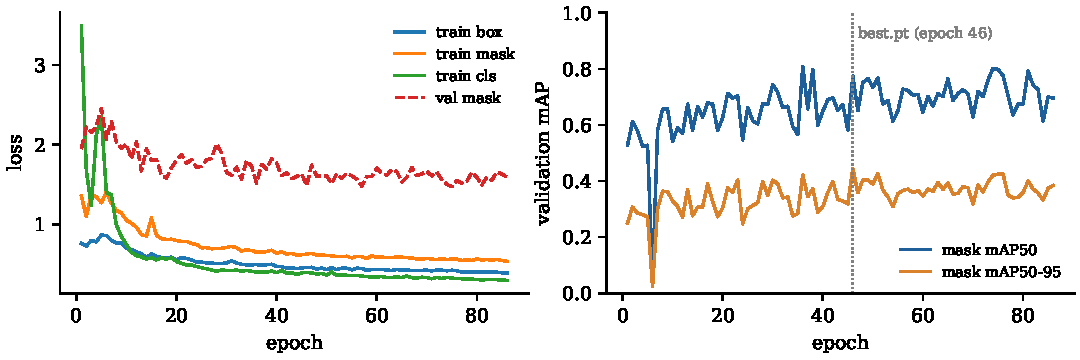
\includegraphics[width=\linewidth]{training.pdf}
  \caption{Training losses and validation mask mAP.}
  \label{fig:train}
\end{figure}

The validation mAP (mask mAP50 = 0.77) is lower than the count accuracy. The reason is that YOLO validates on whole images downscaled to 1024\,px, where the objects are about 2.3 times smaller than at inference.

\subsection{Inference}
\code{AI/count\_objects\_yolo.py} resizes the image to a long side of 2400\,px and predicts on the whole image in one pass. The input size is rounded up to a multiple of 32.
The settings are \code{conf=0.4}, \code{iou=0.5}, \code{max\_det=1000} and full-resolution masks. The count is the number of predicted masks.

% ---------------------------------------------------------------------------
\section{Results}

\begin{table}[H]
  \centering
  \small
  \caption{Mean and worst-image count accuracy (\%) for each split. The AI model never saw the val and test images during training. The Non-AI solution has no training, so for it all splits are unseen data.}
  \label{tab:summary}
  \begin{tabular}{lrrrrr}
    \toprule
    & & \multicolumn{2}{c}{Non-AI} & \multicolumn{2}{c}{AI} \\
    \cmidrule(lr){3-4}\cmidrule(lr){5-6}
    Split & Images & Mean & Worst & Mean & Worst \\
    \midrule
    \tabinput{tables/summary.tex}
    \bottomrule
  \end{tabular}
\end{table}

\begin{figure}[H]
  \centering
  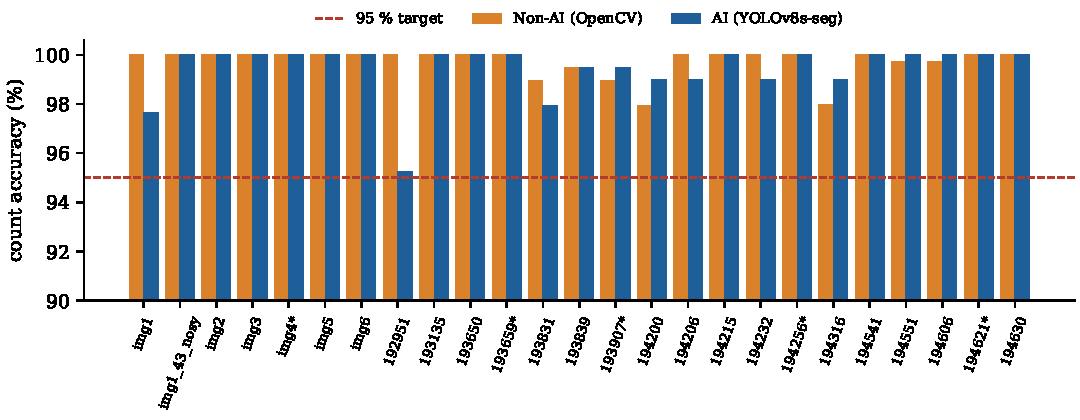
\includegraphics[width=\linewidth]{accuracy.pdf}
  \caption{Count accuracy for each image. Test images are marked with *. Every image is above the 95\,\% target with both methods.}
  \label{fig:acc}
\end{figure}

\begin{table}[H]
  \centering
  \small
  \caption{Counts for each image. ``SAM'' is the automatic label count before human correction.}
  \label{tab:perimage}
  \begin{tabular}{llrrrrrr}
    \toprule
    Image & Split & Ground truth & SAM & Non-AI & Acc.\ (\%) & AI & Acc.\ (\%) \\
    \midrule
    \tabinput{tables/per_image.tex}
    \bottomrule
  \end{tabular}
\end{table}

\begin{figure}[H]
  \centering
  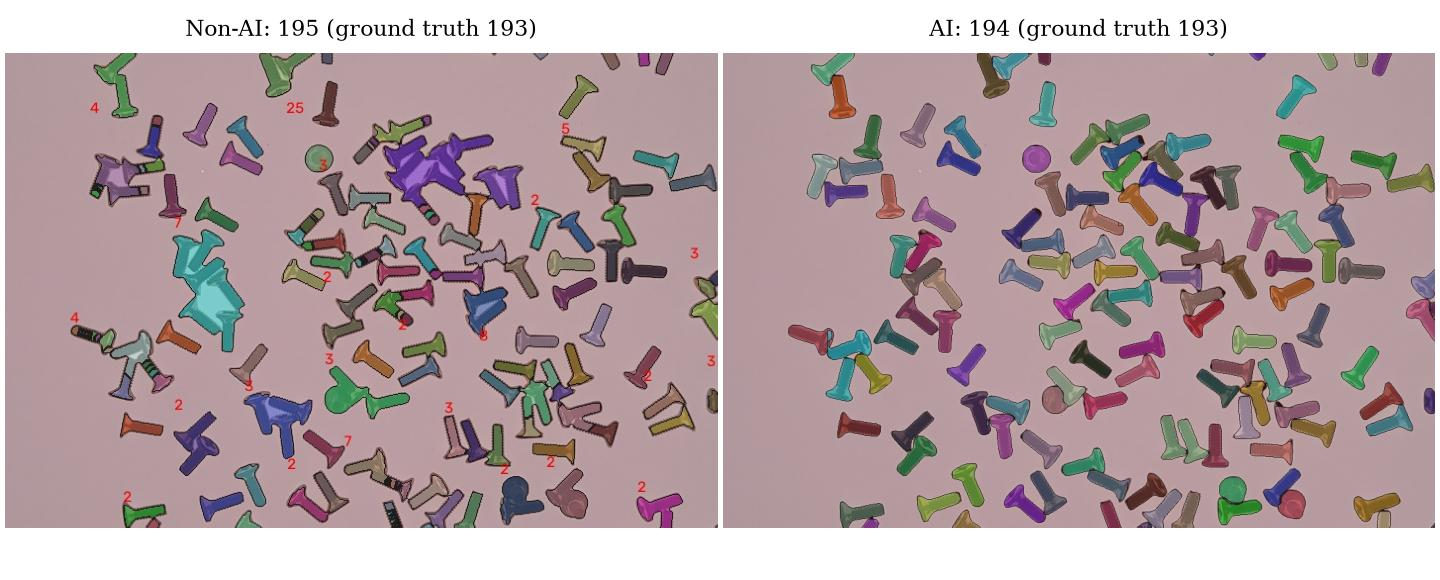
\includegraphics[width=\linewidth]{compare_20240713_193907.jpg}\\[2pt]
  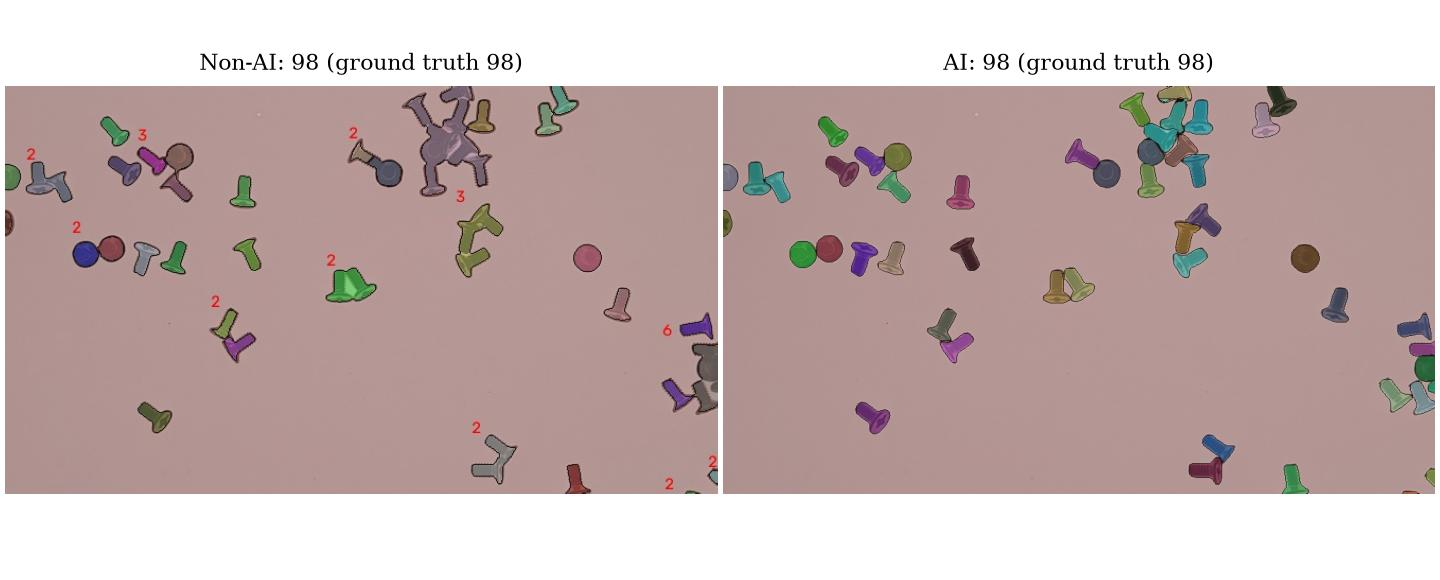
\includegraphics[width=\linewidth]{compare_20240713_194256.jpg}
  \caption{Outputs on two test images (crops): dense screws (top), and screws with discs (bottom). Left: Non-AI. Right: AI.}
  \label{fig:cmp1}
\end{figure}

\begin{figure}[H]
  \centering
  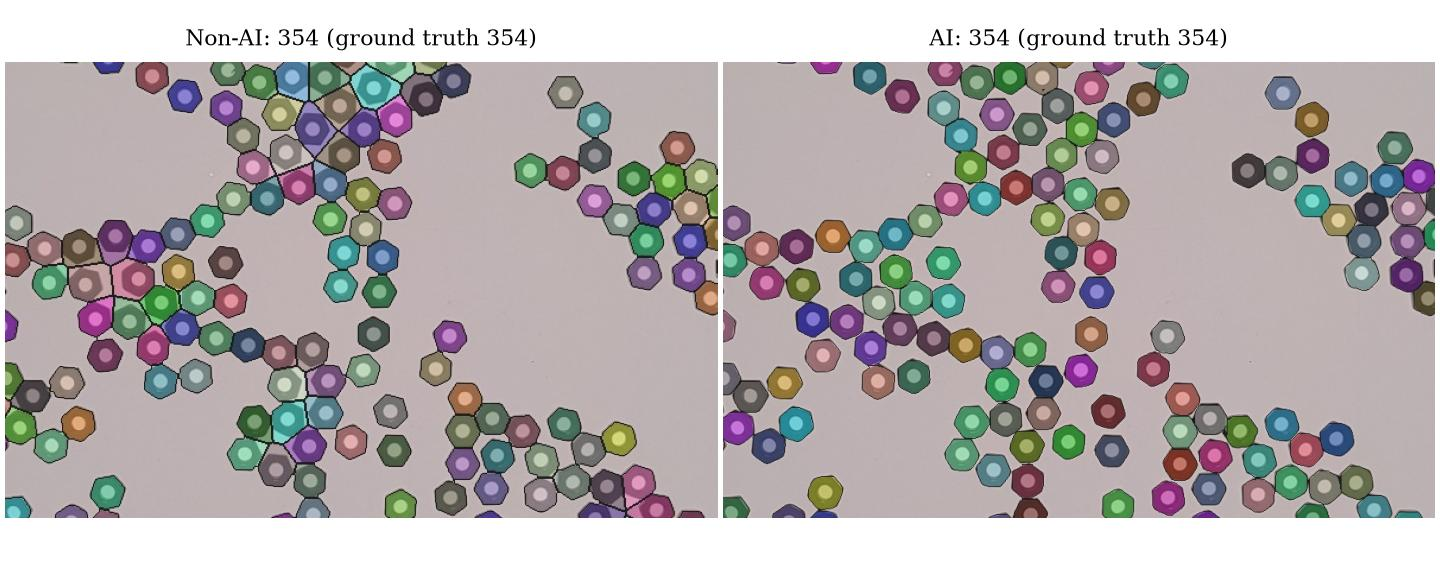
\includegraphics[width=\linewidth]{compare_20240713_194621.jpg}\\[2pt]
  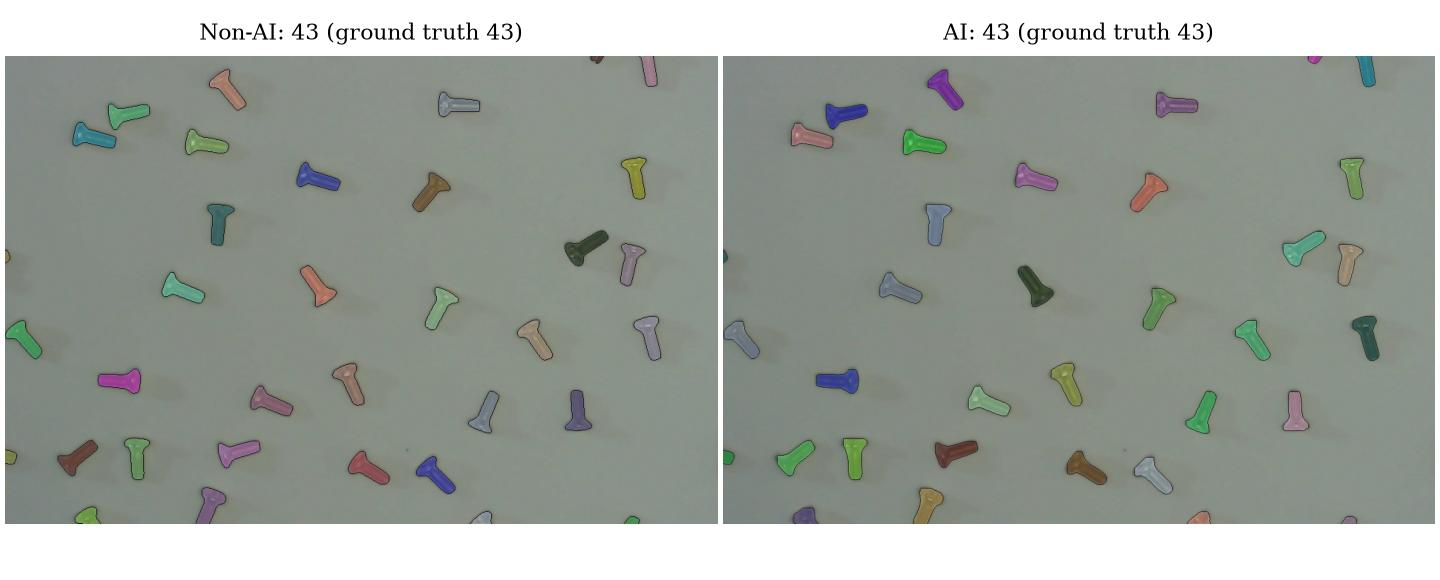
\includegraphics[width=\linewidth]{compare_img4.jpg}
  \caption{Outputs on two more test images (crops): nut pile (top) and sparse screws (bottom).}
  \label{fig:cmp2}
\end{figure}

\section{Discussion}
\begin{itemize}\setlength{\itemsep}{0.2em}
  \item \textbf{Counts.} Both methods are above 95\,\% on every image. Each has its own failure modes. The Non-AI method depends on the area of one object, so it would fail on a scene with no isolated objects. The largest AI error is one extra detection on a sparse training image (22 against 21).
  \item \textbf{Mask quality.} The AI masks follow the object outlines, even inside dense piles (Figure~\ref{fig:cmp1}). The Non-AI watershed counts clusters correctly, but its boundaries inside a cluster are only approximate.
  \item \textbf{Labelling effort.} SAM with the audit made the AI solution possible with very little manual work: 16 clicks for about 3{,}300 objects.
  \item \textbf{Limitations.} The ground truth comes from the same SAM labels that the AI model is trained on, so a systematic SAM error would not show up in the AI test score. The independent checks reduce this risk: the Non-AI counts, the nut-hole counts, and manual review of every flagged spot.
\end{itemize}

\section{Reproducing}
{\footnotesize
\begin{verbatim}
pip install -r Om_Rode/Non_AI/requirements.txt -r Om_Rode/AI/requirements.txt
python Om_Rode/Non_AI/count_objects.py --data data            # Non-AI
python Om_Rode/AI/autolabel_sam.py && python Om_Rode/AI/audit_labels.py
python Om_Rode/AI/apply_corrections.py                         # 16 clicks
python Om_Rode/AI/prepare_dataset.py && python Om_Rode/AI/train.py
python Om_Rode/AI/count_objects_yolo.py --data data            # AI
python Om_Rode/evaluate.py Om_Rode/AI/outputs/counts.csv
python Om_Rode/report/make_figures.py                          # this report
\end{verbatim}
}

\end{document}
